\documentclass[11pt]{article}
\usepackage[margin=0.85in]{geometry}
\usepackage{amsmath,amssymb}
\usepackage[utf8]{inputenc}
\usepackage[T1]{fontenc}
\usepackage[hidelinks]{hyperref}
\usepackage{tikz}
\emergencystretch=3em
\setlength{\parindent}{0pt}
\setlength{\parskip}{4pt plus 1pt minus 1pt}

\title{\textbf{A Brief Derivation of Spacetime}}
\author{Emad Mostaque\\[2pt]{\normalsize Intelligent Internet}}
\date{May 4, 2026}

\begin{document}
\maketitle
\thispagestyle{empty}
\vspace{-1.5em}

\subsection*{The problem}

Why does time have a direction that space does not?

The arrow of time is one of the fundamental open problems in physics. Thermodynamics traces it to initial conditions (Boltzmann, 1872). Cosmology to a boundary condition (Penrose, 1979). Quantum mechanics to measurement (von Neumann, 1932). Each adds structure beyond the equations to break the symmetry.

The arrow was a sign. Space is positive: every distance a sum of squares. Time is positive too: $t > 0$, $c > 0$, $\Lambda > 0$. Both are observed. This paper shows they are one algebra in two signatures.

\subsection*{Six steps from dot product to spacetime}

\textbf{Step 1.\; The metric.}

Space carries a dot product $\langle x, y \rangle = x_1 y_1 + x_2 y_2 + \cdots + x_d y_d$, where $d$ is the dimension. The components are the Euclidean metric $\delta_{ij}$. All distances are positive, no direction is special.

\textbf{Step 2.\; Translations.}

The symmetries of $\delta_{ij}$ are rotations $J_{ab}$ and translations $P_a$. On flat space, translations commute: shifting east then north is the same as north then east.

On a curved surface they do not: walking east then north on a sphere does not return you to the same point as north then east. The failure to commute is curvature. Writing $[P_a, P_b] = P_a P_b - P_b P_a$ for the difference, the three maximally symmetric geometries, those preserving the full rotational symmetry of $\delta_{ij}$, are classified by one number:
\[
[P_a, P_b] = \lambda\,J_{ab}.
\]
$\lambda$ is the curvature. $\lambda > 0$: sphere. $\lambda = 0$: flat. $\lambda < 0$: hyperbolic.

\textbf{Step 3.\; Finiteness.}

The metric $\delta_{ij}$ determines a volume form on each of the three geometries. The sphere $S^d$ is compact and has finite total volume; $\mathbb{R}^d$ and $H^d$ are non-compact with infinite total volume. A normalized measure invariant under the full isometry group requires external structure on $\mathbb{R}^d$ and $H^d$ (a cutoff, boundary condition, or weight function) that $\delta_{ij}$ does not contain. $\lambda > 0$ is forced.

\textbf{Step 4.\; Time.}

The sphere $S^d$ sits in $\mathbb{R}^{d+1}$ as $x_1^2 + \cdots + x_{d+1}^2 = R^2$, with isometry algebra $\mathfrak{so}(d{+}1)$. Wick rotating one coordinate, $x_{d+1} \to ix_0$, takes the sphere to the hyperboloid $x_1^2 + \cdots + x_d^2 - x_0^2 = R^2$ and the algebra to $\mathfrak{so}(d,1)$. Two signatures for the extra direction, two real algebras with the same spatial $\mathfrak{so}(d)$ and the same $\lambda$. The hyperboloid is de Sitter space, with cosmological constant $\Lambda = \tfrac{1}{2}(d-1)(d-2)\lambda$ (in $d=4$, $\Lambda = 3\lambda$). The algebra $\mathfrak{so}(d,1)$ is simple and rigid: by Whitehead, no smooth deformation. The sign of $\lambda$ is fixed by the choice of signature; the magnitude is a scale.

\textbf{Step 5.\; The matrix.}

Realize $\mathfrak{so}(d,1)$ as the antisymmetric matrices preserving $\eta = \mathrm{diag}(+1,\ldots,+1,-1)$ on $\mathbb{R}^{d+1}$. Identify rotations $J_{ij} = M_{ij}$, boosts $K_i = M_{di}$, time translation $P_0 = M_{0d}/L$, spatial translations $P_i = M_{0i}/L$, where $L = 1/\sqrt{\lambda}$. The standard $\mathfrak{so}(d,1)$ commutators give boosts $[K_i, P_j] = \delta_{ij} P_0$ and $[K_i, P_0] = P_i$: an invariant scale, the speed of light $c$, and the Lorentz subalgebra of special relativity. Time evolution is the adjoint action of $P_0$: $[P_0, K_i] = -P_i$ and $[P_0, P_i] = -\lambda K_i$. On each $(K_i, P_i)$ plane, this is a $2 \times 2$ matrix:
\[
\mathrm{ad}(P_0) = \begin{pmatrix} 0 & -\lambda \\ -1 & 0 \end{pmatrix}.
\]
For $\lambda > 0$ the eigenvalues $\pm\sqrt{\lambda}$ are real and distinct, with eigenvectors $\ell_\pm = P_i \mp \sqrt{\lambda}\,K_i$ at eigenvalue $\pm\sqrt{\lambda}$. The flow is hyperbolic:
\[
e^{t\,\mathrm{ad}(P_0)} = \cosh(\sqrt{\lambda}\,t)\,I + \frac{\sinh(\sqrt{\lambda}\,t)}{\sqrt{\lambda}}\,\mathrm{ad}(P_0).
\]
In pure de Sitter, the rate $\sqrt{\lambda}$ is the Hubble constant $H = \sqrt{\Lambda/3}$ (in $d=4$), the observed rate of cosmological expansion.

\begin{figure}[h]
\centering
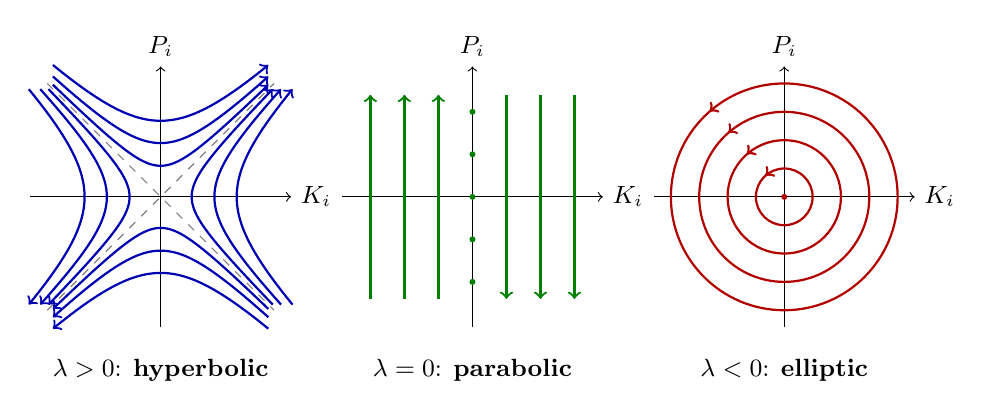
\begin{tikzpicture}[scale=0.72]
\begin{scope}[shift={(-5.5,0)}]
\draw[->] (-2.3,0) -- (2.3,0) node[right] {\small $K_i$};
\draw[->] (0,-2.3) -- (0,2.3) node[above] {\small $P_i$};
\draw[gray,dashed,thin] (-2,-2) -- (2,2);
\draw[gray,dashed,thin] (-2,2) -- (2,-2);
\foreach \c in {0.3, 0.9, 1.8} {
  \draw[->,thick,blue!70!black,domain=-1.9:1.9,samples=80]
    plot ({sqrt(\c + (\x)^2)}, {\x});
  \draw[<-,thick,blue!70!black,domain=-1.9:1.9,samples=80]
    plot ({-sqrt(\c + (\x)^2)}, {\x});
}
\foreach \c in {0.3, 0.9, 1.8} {
  \draw[->,thick,blue!70!black,domain=-1.9:1.9,samples=80]
    plot ({\x}, {sqrt(\c + (\x)^2)});
  \draw[<-,thick,blue!70!black,domain=-1.9:1.9,samples=80]
    plot ({\x}, {-sqrt(\c + (\x)^2)});
}
\node[below] at (0,-2.7) {\small $\lambda > 0$: \textbf{hyperbolic}};
\end{scope}
\begin{scope}[shift={(0,0)}]
\draw[->] (-2.3,0) -- (2.3,0) node[right] {\small $K_i$};
\draw[->] (0,-2.3) -- (0,2.3) node[above] {\small $P_i$};
\foreach \k in {-1.8, -1.2, -0.6, 0.6, 1.2, 1.8} {
  \ifdim \k pt > 0pt
    \draw[->,thick,green!50!black] (\k, 1.8) -- (\k, -1.8);
  \else
    \draw[->,thick,green!50!black] (\k, -1.8) -- (\k, 1.8);
  \fi
}
\foreach \p in {-1.5, -0.75, 0, 0.75, 1.5} {
  \fill[green!50!black] (0, \p) circle (1.5pt);
}
\node[below] at (0,-2.7) {\small $\lambda = 0$: \textbf{parabolic}};
\end{scope}
\begin{scope}[shift={(5.5,0)}]
\draw[->] (-2.3,0) -- (2.3,0) node[right] {\small $K_i$};
\draw[->] (0,-2.3) -- (0,2.3) node[above] {\small $P_i$};
\foreach \r in {0.5, 1.0, 1.5, 2.0} {
  \draw[thick,red!70!black] (0,0) circle (\r);
}
\foreach \r in {0.5, 1.0, 1.5, 2.0} {
  \draw[->,thick,red!70!black] ({-\r*sin(40)},{\r*cos(40)}) -- ({-\r*sin(41)},{\r*cos(41)});
  \draw[->,thick,red!70!black] ({\r*sin(220)},{-\r*cos(220)}) -- ({\r*sin(221)},{-\r*cos(221)});
}
\fill[red!70!black] (0,0) circle (1.5pt);
\node[below] at (0,-2.7) {\small $\lambda < 0$: \textbf{elliptic}};
\end{scope}
\end{tikzpicture}
\smallskip
\begin{center}
\small\textit{How time evolution acts in the $(K_i, P_i)$ plane for each sign of $\lambda$.\\
Only $\lambda > 0$ separates. The other two are shown for comparison.}
\end{center}
\end{figure}

\textbf{Step 6.\; The sign.}

Time evolution is a symmetry of the geometry, so it preserves spacetime length. It scales one eigendirection by $e^{+\sqrt{\lambda}\,t}$ and the other by $e^{-\sqrt{\lambda}\,t}$. A length-preserving flow can scale a vector by $s \neq 1$ only if its length is zero; otherwise the length would change by $s^2$. In spacetime (distance squared minus time squared) some non-zero vectors have zero length: light rays. The eigendirections are light rays. The exponential scaling is the cosmological redshift; the scale factor $e^{\sqrt{\lambda}\,t}$ satisfies the Friedmann equation $H^2 = \lambda$.

One eigendirection grows without bound; this is the future horizon, the cosmological horizon beyond which signals never reach us. The other contracts toward zero; this is the past horizon, the limit beyond which light has not yet arrived. They are different generators in the algebra.

The eigenvalues are signed: $+\sqrt{\lambda}$ and $-\sqrt{\lambda}$. The positive eigenvalue is $t > 0$. It is the sign of cosmological expansion, the sign of $c$, the sign of $\Lambda$. The same sign.

The future is the direction of positive $t$ increase, just as positive $\Lambda$ means the universe expands in time.

$t > 0$.\hfill$\square$

\end{document}
